
\section{Introduction}

Termination continues to be an important theoretical property that is
of practical interest. 
In recent years there has been a proliferation of termination
verification tools, including
{\sc Terminator},
Ultimate,
APrOVE,
and many others
(see SV-COMP)

Unfortunately, current termination tools are limited in two ways.
First, proving termination is {\bf slow}...
point to SVComp results here.
Second, termination tools have limited expressivity 
and are unable to capture termination arguments for 
loops that involve more elaborate mathematical functions
such as trigonometric functions, exponentials, square root, etc.

These kinds of functions are important parts of many applications.
Here is an example, taken from a machine learning algorithm...


Meanwhile, recent advances in learning have lead to classifiers
that are capable of quickly recognizing patterns such as


The main idea of this paper is to accelerate and to expand the expressivity of termination and non-termination proof  techniques, by
incorporating dynamic classification...



\section{Motivating examples}
\newcommand\tx{\texttt{x}}
\newcommand\ty{\texttt{y}}
\newcommand\boxedtt[1]{\fbox{\begin{minipage}{2.5in} #1 \end{minipage}}}
\newcommand\vtrace[1]{{\tt\bf vtrace$_{#1}$}}
\paragraph{Example 1: Linear Termination \& Non-termination.}
Consider the following program:
\begin{center}
  \begin{program}[style=tt]
    wh\tab ile (x >= 0) \{
      x := x + y; \untab
    \}
  \end{program}
\end{center}
Termination of this program depends on the initial values of \tx\ and \ty.
When the initial values of \tx\ and \ty\ are ...

Through a simple transformation, one can instrument each loop
so that the state (values of variables) can be dynamically monitored.
%
As is commonly done in program analysis, we introduce a counter
for each loop~\cite{speed08}. In addition to this counter, however, 
we also introduce a (nondeterministically chosen) \emph{bound} and statements that 
cause the program to exit the loop whenever the counter reaches the bound:
\begin{center}
  \begin{program}[style=tt]
\boxedtt{int \_ctr = 0; int \_bound;
\vtrace{0}(x, y);}
wh\tab ile (x $>=$ 0) \{
  \boxedtt{if (\_ctr $>$ \_bound) break;
  else \_ctr++;
  \vtrace{1}(x, y);}
  x := x + y; \untab
\}
\boxedtt{if (\_ctr <= \_bound) \vtrace{2}(x, y);}
  \end{program}
\end{center}
Alarmingly, this transformation {\bf changes the behavior of the program}.


\[\begin{array}{ll}
\Pi_a =& \{ v0 \cdot v2 \}\\
\Pi_b =& (v0 \cdot (v1)^* \cdot v2)\\
\Pi_c =& (v0 \cdot (v1)^* \cdot bnd)\\
\end{array}\]





\red{relational instrumentation:}
\begin{center}
  \begin{program}[style=tt]
\boxedtt{vtrace0(x, y);
int counter = 0;}
wh\tab ile (x $>=$ 0) \{
  \boxedtt{if (counter $>$ bnd) break;
  else counter++;
  vtrace1(x, y);}

  x0 = x;
  y0 = y;
  x1 = x0 + y0;
  y1 = y0;
  x = x1;
  y = y1;
  vtrace3(x0, y0, x1, y1);
\}
if\tab\ (counter <= bnd) 
  vtrace2(x, y);
  \end{program}
\end{center}



\paragraph{Example 2: Trigonometric functions.}
We now describe a program for which proving termination/non-termination 
escapes known techniques.

Oftne programs, especially scientific applications, terminate due to more complicated mathematical reasons. Example:
\begin{center}
  \begin{program}[style=tt]
    wh\tab ile (y < 42) \{
      y := a * sin(x);
      x := x + 1;
      a := a + 1; \untab
    \}
  \end{program}
\end{center}
sine procedure. terminates when the amplitude goes above threshold of 42.

On the other hand, classification based on dynamic analysis is very powerful and can infer the behavior




\subsection{Key Idea}

\begin{center}
\texttt{while (x>=0) \{ x = x + y\}}

\bigskip
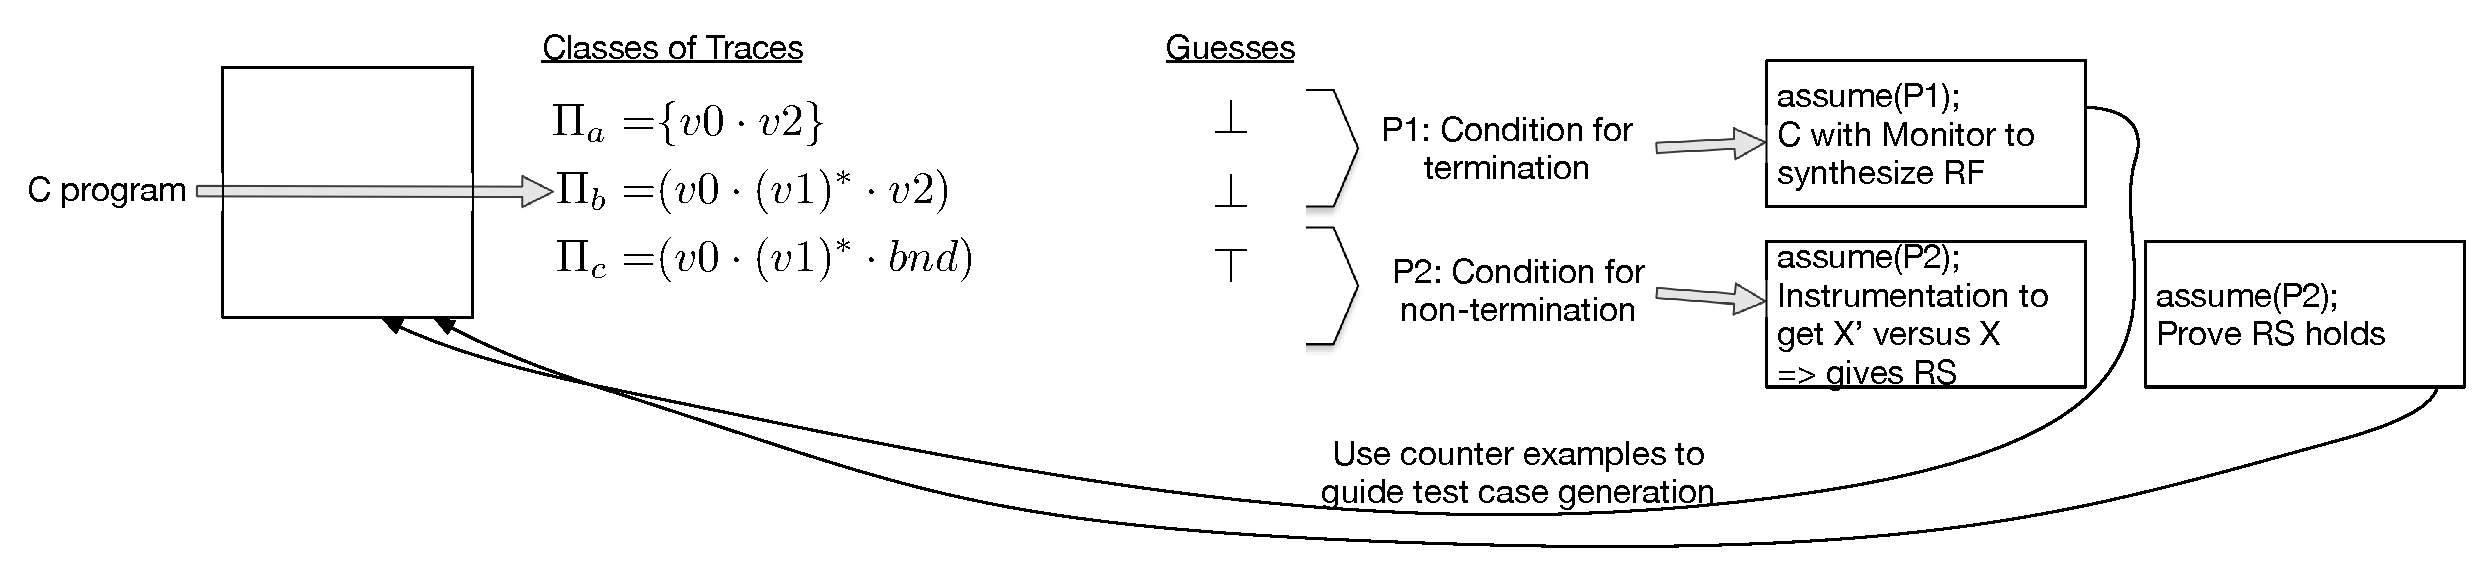
\includegraphics[width=4.5in]{boxes.eps}

\end{center}

\subsection{Expressiveness}

complciated functions like sin, exp, etc.

abstraction
